\documentclass[12pt]{extarticle}
\usepackage[utf8]{inputenc}
\usepackage{graphicx}
\usepackage{float}
\usepackage{hyperref}
\hypersetup{
    colorlinks=true,
    linkcolor=blue,
    filecolor=magenta,      
    urlcolor=blue,
    pdftitle={Overleaf Example},
    pdfpagemode=FullScreen,
    }

\title{CS 3600 Project 2 Wrapper}
\author{CS 3600 - Spring 2022}
\date{Due March 6th 2022 at 11:59pm EST via Gradescope}

\begin{document}

\maketitle

\section*{Introduction}

This Project Wrapper is composed of 4 questions, each worth 1 point. Please
limit your responses to a maximum of 200 words. The focus of this assignment is to train your ability to reason through the consequences and ethical implications of computational intelligence, therefore do not focus on getting ”the right answer”, but rather on demonstrating that you are able to consider the impacts of your designs.

\section*{Context}

Reinforcement learning is a powerful technique for problem-solving in environments with stochastic actions. As with any Markov Decision Process, the reward function dictates what is considered optimal behavior by an agent. Since a reinforcement learning agent is trying to find a policy that maximizes expected future reward, changing when and how much reward the agent gets changes its policy. \\

\newpage

\begin{figure}
    \centering
    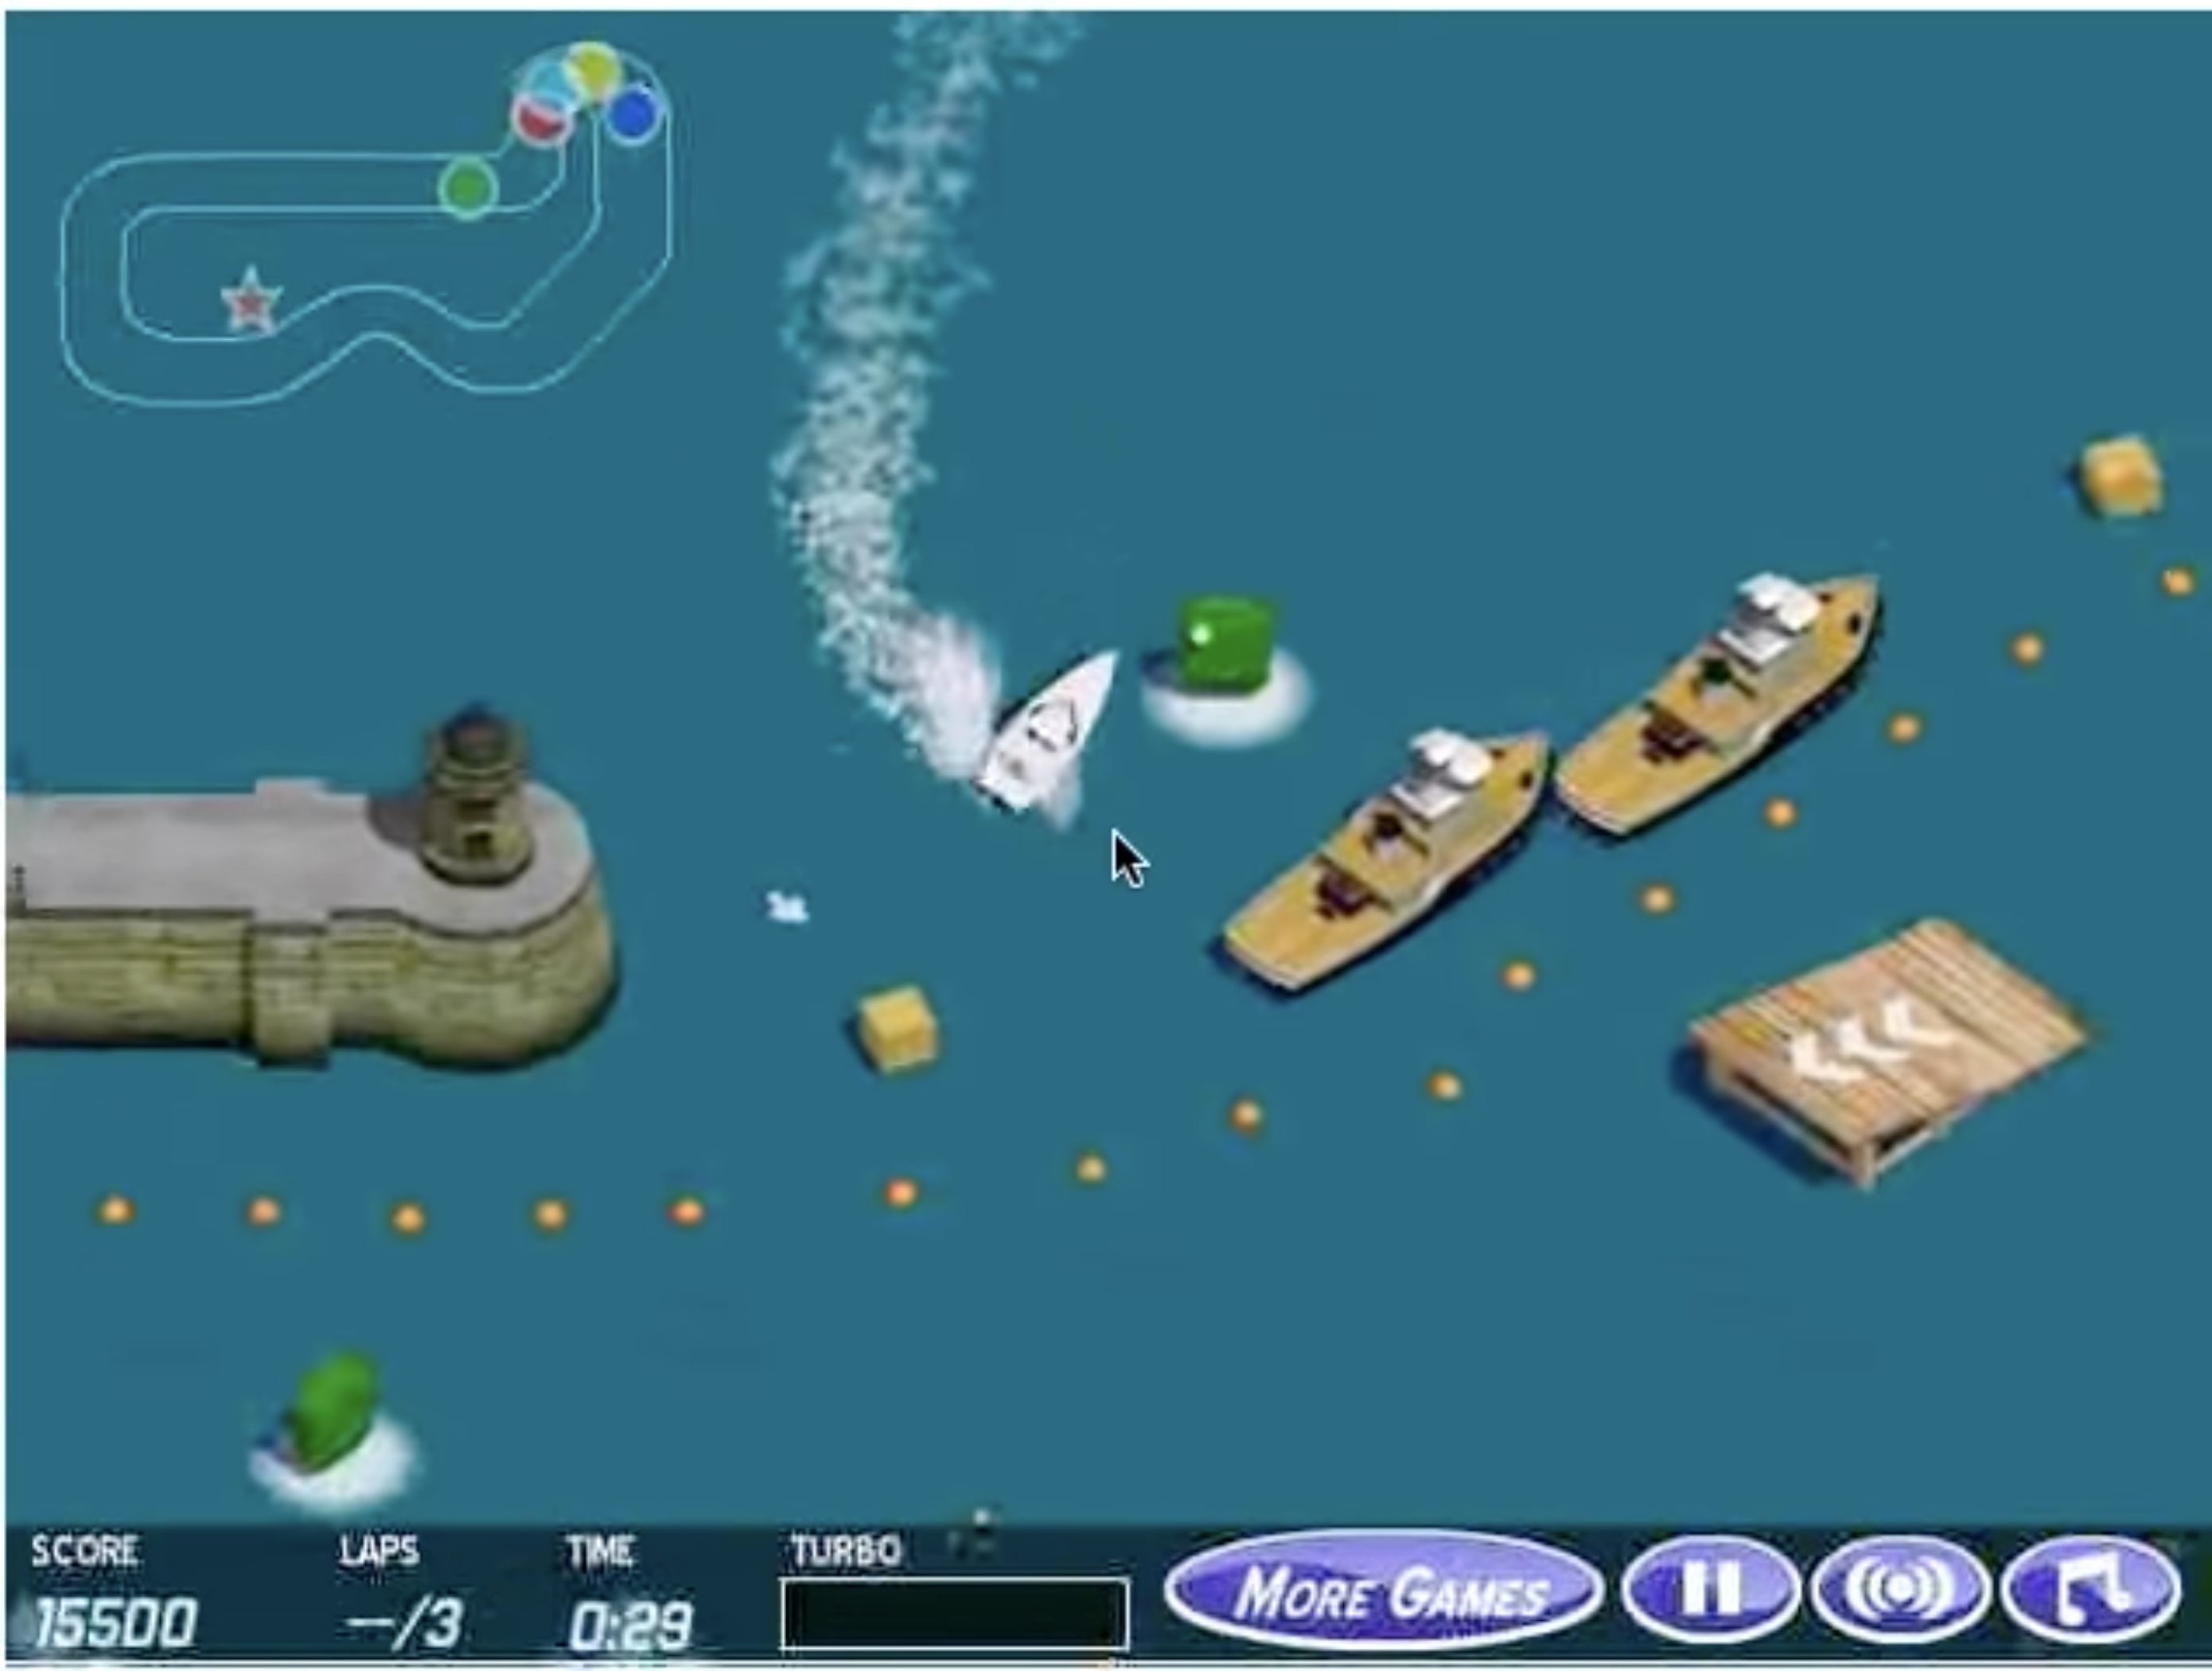
\includegraphics[width=\textwidth]{img/P2WrapperBoat.png}
\end{figure}

\noindent However, if the reward function is not specified correctly (meaning rewards are not given for the appropriate actions in the appropriate states) the agent’s behavior can differ from what is intended by the AI designer. Consider the boat racing game pictured above. The goal, as understood by people, is to quickly finish the race. Humans have no difficulty playing the game and driving the boat to the end of the course. However, when a reinforcement learning agent learns how to play the game, it never completes the course. In fact, it finds a spot and goes in circles until time runs out. You can see the RL agent in action in this video: \href{https://youtu.be/tlOIHko8ySg}{https://youtu.be/tlOIHko8ySg}.The agent’s reward function is the score the player receives while playing the game. Score is given for collecting power-ups and doing tricks, but no points are given to players for completing the course.

\newpage
\section*{Question 1}

Watch the video and explain why the agent’s policy has learned this circling behavior instead of progressing to the end of the course like we expect from a human player. Explain the behavior in terms of utility and reward. \\

\noindent\textbf{Answer:}

\newpage
\section*{Question 2}

When humans play, the rules for scoring are the same. Why do humans play differently then, always completing the course? Why don’t humans circle in the same spot in the course endlessly if they are receiving the same score feedback as the agent? \\

\noindent\textbf{Answer:} 

\newpage
\section*{Question 3}

The agent’s original reward function is:

$$R(s_t, a) = game\_score(s_t) - game\_score(s_{t-1})$$

\noindent Describe in terms of utility, reward, and score \textbf{two} ways one could modify the reward function to get the agent to behave more like a human player. That is, what do we need to change to make the agent complete the course every single time? Assume the agent has access to state information such as the position and speed of the boat and all rival racers, but we cannot change how the game itself provides scores through the call $game\_score(s_t)$. \\

\noindent\textbf{Answer:} 

\newpage
\section*{Question 4}

Self-driving cars do not use reinforcement learning for a variety of reasons, including the difficulty of teaching RL agents in the real world, and the dangers of a taxi accidentally learning undesired policies as we saw with the boat game example. Suppose however, that you tried to make a reinforcement learning agent that drove a taxi. The agent is given reward based on how much fare is paid for the ride, including tips given by the passenger. Describe a scenario in which, after the taxi agent has learned a policy, the autonomous car might choose to do an action that puts either the rider, pedestrians, or other drivers in danger. \\

\noindent\textbf{Answer:}

\end{document}
